\documentclass[a4paper, oneside, draft]{memoir}
\usepackage[T1]{fontenc}
\usepackage[utf8]{inputenc}
\usepackage[english]{babel}

% bedre orddeling Gør at der som minimum skal blive to tegn på linien ved
% orddeling og minimum flyttes to tegn ned på næste linie. Desværre er værdien
% anvendt af babel »12«, hvilket kan give orddelingen »h-vor«.
\renewcommand{\englishhyphenmins}{22} 

\usepackage{colortbl}  % Bruges til at farve celler, rækker mv. i tabeller
\usepackage{pdflscape} % Gør landscape-environmentet tilgængeligt
\usepackage{fixme}     % Indsæt "fixme" noter i drafts.
\usepackage{hyperref}  % Indsæter links (interne og eksterne) i PDF

\usepackage[format=hang]{caption,subfig}
\usepackage{graphicx}

\renewcommand{\ttdefault}{pcr} % Bedre typewriter font
%\usepackage[sc]{mathpazo}     % Palatino font
\renewcommand{\rmdefault}{ugm} % Garamond
%\usepackage[garamond]{mathdesign}

%\overfullrule=5pt
%\setsecnumdepth{part}
\setcounter{secnumdepth}{-1} % Sæt overskriftsnummereringsdybde. Disable = -1.
\chapterstyle{hangnum} % changes style of chapters, to look nice.

\makeatletter
\newenvironment{nonfloatingfigure}{
  \vskip\intextsep
  \def\@captype{figure}
  }{
  \vskip\intextsep
}

\newenvironment{nonfloatingtable}{
  \vskip\intextsep
  \def\@captype{table}
  }{
  \vskip\intextsep
}

\makeatother


\newcommand{\EDSL}{EDSL (Embedded Domain Specific Language) \renewcommand{\EDSL}{ EDSL }}

\title{Controlling embedded devices with functional reactive programming}

\author{Martin Dybdal (dybber@dybber.dk), \\
Jesper Reenberg (jesper.reenberg@gmail.com) \\ og
Troels Henriksen (athas@sigkill.dk)}

\date{\today}
\pagestyle{plain}



\begin{document}

\maketitle

\begin{abstract}
  Robots are conventionally programmed in low-level imperative
  languages with no concepts like events, synchronicity or any of the
  advantages found in functional programming languages (like pattern
  matching). Reactive programming languages embedded in Haskell, like
  Frob \cite{frob99} and Yampa \cite{arrowsrobotsfrp02}, has been
  suggested for robot programming, but they require a complete Haskell
  runtime system, which is to large to fit on more
  resource-constrained devices. 

  We tie these two ends together, creating a highly declarative
  language for robot programming using a staged compilation-strategy
  like the one found in Flask \cite{flask08}, that makes it possible
  to run programs on devices with few resources. In the creation we've
  used the Flask-codebase as a starting point and huge parts of the
  code is left unchanged.
\end{abstract}

\clearpage 

\tableofcontents*

\fixme{remove all uses of "`very"'}
\fixme{change bibtex style to one that includes URL's in the generated list,
  such as plain-url or another fancy one.}
\fixme{change $\backslash$ url to use the hyperref package so real links are
  used.}
\fixme{check all quoted text for use of the same quotes!!!!}


\chapter{Disposition}
\begin{itemize}
\item Abstract

\item Preface

\item Introduction
  \begin{itemize}
  \item Brief intro to robot programming
    \begin{itemize}
     \item Sensors and Actuators
    \end{itemize}
  \item Brief Arduino introduction
  \item Brief Flask introduction
    \begin{itemize}
     \item The staged compilation strategy
    \end{itemize}
  \end{itemize}

\item Related Work
  \begin{itemize}
  \item Frob
  \item Esterel
    (http://www.softwaresafety.net/Esterel.org/esterel.html)
  \item Lustre \cite{lustre91}
  \item Flask
  \end{itemize}

\item "`Our system"'
  \begin{itemize}
  \item Staged compilation
  \item Dataflows
  \item Node representation
  \item Devices
  \item Interrupts
  \item Events
  \end{itemize}

\item Example programs

\item Conclusions

\item Bibliography

\item Appendixes
  \begin{itemize}
  \item A Flask tour
  \item Small guide to Arduino and electronics
  \end{itemize}
\end{itemize}  



\chapter{Preface}
This paper is written as a 15 ECTS Bachelor project at the Computer
Science Department (DIKU), University of Copenhagen. The authors are
Martin Dybdal, Troels Henriksen and Jesper Reenberg. The project is
supervised by Ken Friis Larsen, assistant professor at DIKU.

\fixme{maybe add thanks to Flask-guys}


\chapter{Introduction}
Robots has been used in the industry for decades, replacing humans in
repetitive tasks like sewing, assembling and transportation. In the
last years smaller robots like the Roomba vacuum cleaner has been
introduced to the consumer market, which is a sign that robots are
getting cheaper an affordable for more tasks. We will probably see
robots deployed in many other uses.


Electronics is replacing more and more devices that has been
controlled mechanically before. 


Production cost falling => cheaper robots => more robots to be
programmed. Fast prototyping and re-usability are important for the
industry.

....

First we establish how the domain of reactive systems is
identified. We've found the best description in Zhanyong Wan's PhD
thesis "`Functional Reactive Programming for Real-Time reactive
systems"'. \fixme{make this a latex-cite}. As he explains we can
partition computer systems into:
\begin{itemize}
\item Transitional systems, that takes some data as input, does some
  computation on it and delivers some resulting output (an example of this
  is a compiler).
\item Interactive systems, where the state of the program switches
  from computation to getting more input and back (a text editor is an
  example).
\item Reactive systems that continuously has to respond to
  environmental changes. Often reactive systems has to do with our
  physical environment, either simulating it (e.g. a computer game) or
  is required to respond to its changes (e.g. a robot).
\end{itemize}





We think that functional reactive programming using a dataflow-based
approach looks like a good candidate for programming these systems...


\fixme{evt. forklaring af "`reactive programming"'. Se }

\chapter{Flask}
Flask is a domain specific language embedded in Haskell for
programming sensor networks. A fundamental thing in when learning
Flask is understanding its compilation-strategy. The basic idea is to
use Haskell as a metalanguage for several object languages, and
generate a code in a sensor network language called NesC\footnote{NesC
  is an extension to C, with some additional constructs suitable for
  low-level sensor network programming for TinyOS.} when running the
Haskell program. The generated NesC code can then be translated by an
ordinary compiler NesC compiler to machine code running on the nodes
in the sensor network.

\begin{nonfloatingfigure}
  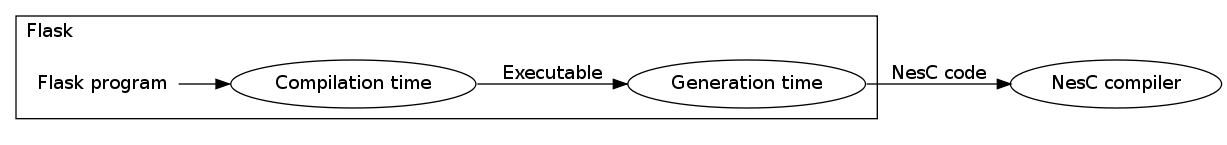
\includegraphics[width=0.9\textwidth]{images/flask-simple}
  \centering
\end{nonfloatingfigure}

Thus, when you write a Flask-program, you use ordinary Haskell
constructs to manipulate which NesC-code should ultimately be
generated. A program is a description of the flow of data from inputs
(e.g. hardware sensor) to outputs (e.g. another node) in the specific
sensor node. The description takes the form of an acyclic graph
connecting inputs to outputs, with some optional processing in
between. For specifying this \textit{dataflow graph}, Flask provides
some general \textit{signal functions} that can be combined with
\textit{node-level code} (code that is actually getting to run on the
sensor-nodes) written in one of the object-languages.

Example dataflow graph from the Flask paper: 

\begin{figure}
  % ewma example
\end{figure}

Flask provides two object-languages: NesC and Red. Having NesC as an
object-language, allows the user to write all programs that's
expressible in NesC. Red is an amputated Haskell, without recursion,
recursive datatypes, most of the standard library and curried
functions. It allows you to write concise functions for simple tasks
instead of having to deal with NesC. The reason for disallowing these
things are the same as for not compiling Haskell directly to the
sensor nodes in the first place: the Haskell runtime is too huge to
fit in the limited memory of a sensor node.

Both languages are integrated into Flask using the quasiquotation
library \cite{quasiquote07}, also written by the Flask author. This
allows you to write the object languages in their original syntax
inside the Flask/Haskell environment. And it allows you to intersperse
generation time variables (which results in compile time constants)
into to object language code.


... 

More on:
  Typechecking
  Dataflow




\chapter{Overview of the Fladuino system}

Fladuino is a modification of Flask that can be used to program
Arduino devices in a functional reactive manner.

\section{A note on Arduino}

The term ``Arduino'' is somewhat ambiguous.  It is both a registered
trademark of the Arduino team that can be used by licensed
manufacturers, a line of platforms based on various Atmel AVR
microcontrollers, as well as a general term for any device that is
mostly compatible with the official Arduino microcontroller boards.
This paper will use the latter meaning unless otherwise is explicitly
mentioned.

Additionally, we have only had resources to test our work on the
Arduino
Duemilanove\footnote{\url{http://www.arduino.cc/en/Main/ArduinoBoardDuemilanove}},
Arduino BT\footnote{\url{http://www.arduino.cc/en/Guide/ArduinoBT}},
Arduino
Mega\footnote{\url{http://arduino.cc/en/Main/ArduinoBoardMega}},
and Pololu 3pi\footnote{\url{http://www.pololu.com/catalog/product/975}}.

\section{Terminology and basic \textit{modus operandi}}

As in Flask, Fladuino is implemented as a set of Haskell modules that
provides facilities for expressing the structure and behavior of a
\textit{dataflow graph}, connecting \textit{dataflow operators}
through value-carrying directed graph edges (\textit{wires}).  The
programmer writes a Haskell program, called the \textit{generator
  program}, or just the \textit{program}.  We shall refer to the
compilation of the program as \textit{compile--time}, and execution of
the program as \textit{generation--time}.  At generation--time, the
output will be a program source file suitable for further compilation
with the Arduino tools, but these are not part of the Fladuino system.
Generation--time may also terminate erroneously if the program
contains static errors: in this case, an error message with a
description of the problem will be printed.  Only errors that are
violations of the Haskell type system can be caught at compile--time,
and while we have attempted to structure the facilities provided by
Fladuino such that invalid programs will contain type errors, this
cannot be done for all error classes.

\fixme{We ought to have a little description of which types of errors is caught
  at which point. Seems a little quick to mention it but not to clarify}

\section{Structural overview}

Fladuino consists of several interconnected parts combined to form a
domain-specific language embedded in Haskell.\footnote{We do however
  make heavy use of Glasgow Haskell language extensions, such as
  multi--parameter typeclasses and existential types, so Fladuino will
  not run in a standard implementation of Haskell 98.}  As in Flask,
this takes the form of providing facilities to express the structure
of a \textit{dataflow graph}, connecting \textit{dataflow operators}
through directed graph edges (\textit{wires}).  Conceptually, these
parts can be divided into the following:

\begin{itemize}
\item Haskell operators and functions used to describe the dataflow
  graph have been defined.  It is not intended that these are
  exclusively used to construct the program, but rather that they are
  part of a larger Haskell program.  Since a Fladuino program is
  highly static at run-time, the generating program should be written
  to support easy configuration and modification.  In a very real
  sense, the dynamic part of a Fladuino program happens at
  compile--time.
\item A compiler is supplied for the Haskell-like programming language
  Red, which is used to tailor the behavior of stream operators.
\item A module that encapsulates the hardware facilities offered by
  the target platform and provides the ability to check whether the
  requirements made by the users program can be fulfilled.  Arduino is
  a highly variable hardware platform, no more than a simple
  microcontroller connected to a basic extensible circuit board, and
  no assumptions can be made about which electrical components the
  user might need to control.  Therefore we provide a comprehensive
  facility for expressing device interaction in a high-level fashion,
  and automatically check whether any of these interactions are
  incompatible, or violate basic hardware restrictions.  For example,
  we might check that the program does not try to interact with a
  pushbutton connected to a hardware pin that does not support
  interrupts, or that the program does not express both a
  potentiometer and diode connected to the same pin.\footnote{Of
    course, it must be mentioned that we cannot possibly check that
    the hardware has actually been set up in the way described by the
    program --- we can only check for internal consistency and
    violations of basic hardware restrictions, not whether the
    programs model of the device actually corresponds with reality.}

  Furthermore, since there are several different boards under the
  Arduino name, all with slightly different capabilities, we permit
  selection of the exact Arduino variant targeted by the program.

  Finally, since Arduino is a fundamentally extensible platform, we
  provide facilities for implementing \textit{drivers} for entirely
  new devices, such that use of these is also automatically
  sanity-checked.
\end{itemize}

\section{Dataflow evaluation strategy}

As in Flask, the dataflow graph is divided into \textit{atomic
  subgraphs} consisting of a set of nodes connected by normal wires.
Evaluating such a subgraph consists of supplying a value on the input
wire, retrieving any values that may show up on output wires, then
setting up to evaluate any of the successor atomic subgraphs with
these values (see \ref{dataflowtranslation} for the implementation
details).  The notion of an atomic subgraph serves the purpose of
dividing the dataflow graph into parts that can be evaluated
atomically without blocking.  While this is conceptually and
implementation--wise simple, it leaves open the question of what to do
with the asynchronous events that are the heart of reactive
programming.  Since events are fundamentally connected to the concept
of a hardware interrupt (though we do not reject the ability for sinks
to manually signal events), we cannot at any time predict, or control,
their arrival.

The simplest strategy would be to, upon arrival of an event via an
asynchronous hardware-level interrupt, immediately evaluate all atomic
subgraphs that have nodes listening to the event.  However, this
approach is unacceptable for several reasons:

\begin{itemize}
\item If we are already in the progress of computing an atomic
  subgraph $s_1$ already, we will have to store information about the
  computation while we evaluate all graphs $s_n$ listening to the
  newly arrived event.  The size of this information can be
  significant, especially if we receive yet another event while
  evaluating one of $s_n$.  There is no upper bound on the number of
  events we can be forced to handle within each other, and the storage
  spent on saving the state of each computation can be very
  significant on such memory-constrained devices as the Arduino
  platform.
\item Doing large computations (in space or time) within interrupt
  handlers is generally a bad idea.  Not only are additional
  interrupts disabled while running the handler (and making them
  re--entrant is nontrivial), but the already running code may already
  tie up an arbitrary amount of the memory resources.  As a result,
  interrupt handlers should ideally terminate swiftly and use very few
  resources, which cannot be guaranteed for evaluation of arbitrary
  atomic subgraphs.
\item Most importantly, the subgraph computation already in progress
  may be in a critical section, and we cannot guarantee that the
  subgraphs to be evaluated in response to the event will not overlap
  with this critical section.  Thus, we can end up with interleaved
  access to explicit state (memory contents) as well as implicit state
  (output).  This violates one of the basic tenets of atomic
  subgraphs, namely atomicity of computation.
\end{itemize}

As a result, our basic program evaluation is as follows.  We maintain
an ordered \textit{event queue}, each element containing information
about an atomic subgraph (actually, an entry node to the subgraph)
that should be called, as well as the input value that caused the
input wire to fire.  The generated program consists of a loop that
continuously checks for the presence of an element in the queue, and
if so, removes it and computes the subgraph indicated by it.  Hardware
interrupts are handled by checking all events that may be signalled by
the given interrupt (the details of this check are defined
individually by each type of event), and if the check is positive, an
element is added to the event queue requesting the evaluation of all
listeners of that event.  It is important that the event--check, as
well as the computation of the value of the event, is done in the
interrupt handler itself, as the value may depend on the hardware
state (such as the voltage on an input pin) as of that moment, and it
cannot be guaranteed that this state will not have changed by the time
the main loop retrieves the element from the event queue.  This means
that we cannot provide any strict guarantees about the resource usage
of interrupt handlers, but this is a hardware issue that is
fundamentally unsolvable in software.  Optimisations can be performed,
of course, but ultimately there are constraints on how much any
computer can do.

\subsection{Details of the event queue}

The event queue itself is such a central cog in our event-pumping
machinery that it is worth paying great attention to its form.  It is
essentially just a double-ended queue, but as it turns out, the
textbook implementation of this data structure is undesirable in
Fladuino.  Normally, one would construct a double-ended queue as a
linked list or array\footnote{In Fladuino, we would use a linked list
  rather than an array, as reserving large contiguous blocks of memory
  on the heap will often not be feasible on the memory-constrained
  Arduino platform.}, requesting additional memory from the heap as
necessary, but this runs the risk of the event--queue ballooning to
great size, especially if the program has an input source that
constantly triggers new events every few milliseconds.  Since the
stack and heap share the same memory space, we would run the risk of a
collision, causing data corruption possibly severe enough to
completely crash the program (eg. if the procedure return address on
the topmost stack frame was modified).  While we could modify the
event queue to perform a check for imminent collision whenever an
element was about to be added (and if so, ignore the event), we cannot
do the same whenever we expand the program stack, so we would run the
risk of the stack growing across the event queue and corrupting its
data, causing great harm when the main loop gets around to processing
these now invalid elements.  In conclusion, we cannot permit the stack
to grow uncontrollably.  An additional problem with using dynamic
memory is the unpredictable runtime behavior of \texttt{malloc()},
something that is undesirable in an interrupt handler, as described in
the preceding section.

The design of our event queue thus has the following constraints:

\begin{itemize}
\item There must be a limit on the amount of memory it can occupy.
\item It must not waste too much memory.
\item Adding an element must have a predictable (and low) runtime
  cost.
\end{itemize}

The third constraint also prevents us from being too clever for our
own good, and for example storing the event-queue in the EEPROM
available on all Arduino variants in order to avoid using the same
memory as the program stack.  While an interesting idea, EEPROM writes
require unacceptable multi-millisecond delays.

Thus, our event queue consists of a statically allocated
(compile--time fixed-size) array that is not too big, and in which
element insertions have hard real-time runtime guarantees.  If an
attempt is made to insert an element into a full event queue, the
result will be a silent failure.  This is a tradeoff: as mentioned in
a previous section, we have to accept that it is possible for the
Arduino to be swamped with more work per time unit (or asked to store
more data) than it is physically able to do.  All we can do is to
design Fladuino such that the fatal error conditions are rare, and the
most common error conditions are survivable.  Stack (or heap)
corruption will in most cases result in the complete malfunction of
the program, and are thus the least desirable error case.  In
Fladuino, use of the heap is very limited (and in fact bounded by the
static maximum size of the event queue), and stack/heap corruption
will in practice only occur if the program is large enough to consume
all available memory with its stack.  The most common error case, on
the other hand, will be attempting to add an element to a full event
queue, resulting in a silent failure.  There are many cases where this
is not desirable, of course, but many reactive programs will not
experience catastrophic failure if they lose even important events,
such as button presses.  Still, we recognise that not all event loss
can be brushed aside as merely an unimportant UI deficiency, and
therefore we provide a facility, termed \textit{idle waiters}, meant
to reduce the average load on the event queue and reduce the risk of
filling it up.

\subsection{Idle waiters}

For many embedded applications, a typical workflow would be to
continuously poll an input source (such as a sensor), then adjusting
some output device based on the reading.  For example, a
line-following robot may take readings from its light sensors, then
adjust its servo--motors to ensure that it is following the line
straightly.  This can be done by simply attaching a node to a clock
that fires every millisecond, but this approach has a notable
disadvantage if many other events are being received at the same time.
The event queue may become filled with a large amount of clock events,
thus drowning out (and losing) potentially more interesting events.
In most cases, it is not a problem that the continuous polling of the
input source is in irregular intervals, but the silent loss of events
such as button presses is normally undesirable.

Thus, we provide the notion of \textit{idle waiters}, a list of atomic
subgraphs that are evaluated in a round--robin fashion whenever the
event queue is empty.  They are a useful facility for specifying
computations that should be done whenever the program is not busy with
something else.

\section{Framework for specifying peripheral drivers}
Arduino is a flexible system for general embedded development, with no
specific application in mind.  The Arduino platform can therefore be
connected to a diverse amount of peripheral devices, all with their
own specific functionality and programming interface.  It is thus
natural to support this diversity as a core concept of Fladuino; not
(solely) as a library of drivers for various devices, but rather as a
framework and set of tools provided to the programmer so that Fladuino
can be extended to transparently support the devices he has need of.
For demonstration, we have \fixme{not really done yet} written a
framework for programming the Pololu 3pi robot and the peripherals
connected to it (electromotors, sensors, buttons, etc.).

Furthermore, Arduino is a broad term encompassing a range of
more-or-less compatible platforms, though each of them differ slightly
in their exact capacity.  Apart from variations in such things as
memory size, they differ in amount and capability of their I/O pins.
This latter diversity is what we are most concerned with in Fladuino,
as we would like to statically check (at generation--time) the
hardware assumptions expressed in the program.  Thus, we also provide
a facility for describing the exact capabilities of a specific
Arduino-based platform, and provide default descriptions of common
Arduino--compatible such as the Arduino Duemilanove, Arduino Mega,
Arduino BT, and Pololu 3pi.

Defining the driver for each external component consist of a general
device specification, a set of functions operating on the device and
eventually some event specifications if the device can generate
some notion of events.

\fixme{find a good example to add here}

\subsection{Platforms}

A platform is defined by a list of \textit{analog pins},
\textit{digital pins}, and free--form \textit{capabilities}, the
latter being a set of strings describing the identity or unusual
qualities of the platform.  For example, the platform definition for
the Pololu 3pi robot contains a ``3pi''--capability that exists merely
to express the fact that the platform supports the quirks of the 3pi
robot that cannot be expressed through a list of pins.  Any device
intended to make use of these quirks would explicitly require the
presence of this capability.

\subsection{Devices}
A device is any form of peripheral that can be connected to the
Arduino robot, e.g. buttons, electromotors and potentiometers.  A
description of a device consists of instructions on how to initialize
such a device and a way of uniquely identifying a device, so we can
have a way of referring to the specific device.  If the device is used
in more than one place, the unique identifier is also used to avoid
adding the initialization code twice.

\subsection{Events}
Some devices can generate events.  The simplest example is the push
button which generates events both when pushed and released.  ...

\chapter{Implementation}

The essence of Fladuino can be condensed to a single, conceptually
simple problem: translate a high-level functional reactive program to
a form suitable for execution on the Arduino platform.  We have chosen
to stop a step short, and merely generate C code meant for further
compilation through an Arduino-specific compiler.  We have no need of
the additional power we would gain through generating our own machine
code, and the additional amount of work required would be very large.
Flask chooses the same approach, in that it produces NesC--code for
running on sensor motes, likely for the same reasons.

Our target platform, Arduino, imposes constraints on the resulting
device-level code.  In particular, the low amount of available main
memory, and the comparatively large amount of available flash memory
for program code, suggests that we optimise for low memory usage over
low code size.  Indeed, as we shall see, we have opted to directly
express much of the control flow in the code itself, where a typical
program, with plenty of available memory, might instead choose a more
data-driven approach.

\section{Basic dataflow translation}
\label{dataflowtranslation}
At their heart, both Flask and Fladuino--programs consist of an
acyclic dataflow graph.  A core part of the system involves the
translation of this high-level description of the passage of data into
the procedural target environment.  Fladuino adopts Flask's
implementation almost verbatim, the details of which will be explained
within this chapter.

As in Flask, the graph is divided into \textit{atomic subgraphs},
sections that can be executed without blocking

\subsection{Translation of a simple dataflow graph}

A set of nodes (dataflow operators) connected by a set of directed
graph edges (wires) make up the entirety of the dataflow graph. Each
wire is associated with type information regarding the values that
will be passed along it.  Some dataflow operators have no predecessor
and exist solely as entry points for data (they can be triggered by
outside events, such as device or timer interrupts), while others have
no successors and function as data sinks.  It is required that the
graph is acyclic, something that is enforced by every operator being
uniquely identified by (among other things) its predecessor(s).  A
stream operator can have multiple distinct input, but only a single
output, though this output can be split so as to send the same output
value to any number of successors.

For every operator $o$ in the dataflow graph, a set of unary
functions $o\_in_n()$ and a unary function $o\_out()$ will be
generated.  The arrival of a value $v$ at $o$ will be implemented by a
call $o\_in_n(v)$, where the exact choice depends on the wiring of the
graph.  In the typical case, even when several wires leads to a single
stream operator, there will be only a single such $o\_in_n()$
function\footnote{In fact, multiple ``in'' functions are only
  necessary for operators such as \texttt{szip}, which works by
  waiting until it has received two values $x, y$ from its two direct
  predecessors, after which it sends them along to its successors as
  the tuple $(x,y)$ --- in this case, the two functions will need
  different types and semantics, as there it is not required that $x$
  and $y$ have the same type.}.  Depending on the specific semantics
of $o$, a value $v'\equiv f(v)$ (where $f()$ represents the
computation done by $o$, the result may not even depend on $v$ at all)
may be propagated to the successors of $o$.  In this case,
$o\_in_n(v)$ will call $o\_out(v')$, the implementation of which will
feature the calls $\forall s \in S(o). s\_in(v')$, where $S(o)$ is the
set of all successors of $o$.

$o\_in()$ is generated directly by the implementation of the specific
dataflow operator, but $o\_out()$ is automatically created by Fladuino
during code generation.  The utility of this division is that the
implementation of a dataflow operator does not feature tedious
duplication of the value propagation machinery, yet as it is not
required that $o\_out()$ is called at all, each dataflow operator can
still make its own choice whether to propagate a value or not.

It is worth nothing that a value need not contain any information
apart from its existence; \texttt{()} is perfectly valid as a signal.


\bibliographystyle{bibliography/theseurl}
\bibliography{bibliography/rapport}

\appendix

\chapter{Small guide to Arduino}

\fixme{We should update the $\backslash$ texttt to uses the listings
  inline formatting instead when ever c code is listed.}

Description of Arduino from the official
website\footnote{\url{http://www.arduino.cc/} downloaded the 28. of April 2009 at 15:16}:
\begin{quotation}
  Arduino is an open-source electronics prototyping platform based on
  flexible, easy-to-use hardware and software. It's intended for
  artists, designers, hobbyists, and anyone interested in creating
  interactive objects or environments.

  Arduino can sense the environment by receiving input from a variety
  of sensors and can affect its surroundings by controlling lights,
  motors, and other actuators. The microcontroller on the board is
  programmed using the Arduino programming language (based on Wiring)
  and the Arduino development environment (based on
  Processing). Arduino projects can be stand-alone or they can
  communicate with software on running on a computer (e.g. Flash,
  Processing, MaxMSP).
\end{quotation}

\begin{nonfloatingfigure}
  \centering
  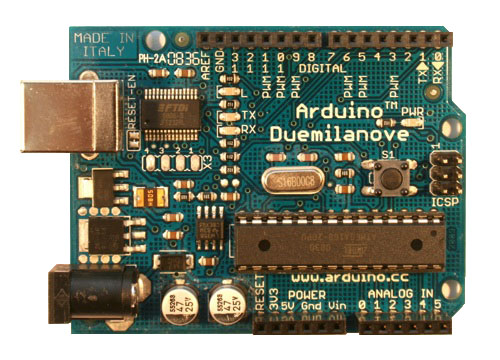
\includegraphics[scale=0.5]{images/ArduinoDuemilanove}

  \caption{Picture of a Arduino Duemilanove. Picture is taken from the Arduino
    homepage: \url{http://arduino.cc/en/Main/ArduinoBoardDuemilanove}.}
  
\end{nonfloatingfigure}

There are different kinds of Arduino boards. All are based on
different ATmega processors from Atmel. The older boards used serial
communication while the newer ones are connected to the computer
through a USB cable, but still using the same serial communication
protocol (i.e. serial through USB). The USB cable also serves as a
power supply.



We will describe the Arduino Duemilanove board we have used, in the
sections that follow, but most information will apply to
the other Arduino boards as well.

\section{Pins}
The Arduino board can connect to several external components through
diverse input and output pins. The pins are split in three physical sections on
the board \textit{power}, \textit{analog in} and
\textit{digital}. Before any IO can happen on a pin, it's mode must be
set. The mode of a pin defines if it is used to read input or
write output. The mode is set by the function \texttt{void pinMode(int
  pinnumber, int mode)} where \textit{pinnumber} is a number between
0-5 for analog and 0-13 for digital and \textit{mode} is either of the constants
\texttt{OUTPUT} or \texttt{INPUT}.

\subsection{Power pins}
% http://arduino.cc/en/Reference/Board?from=Guide.Board
\begin{itemize}
\item Reset: Resets the board when connected to ground.
\item 3V3: Constant 3,3v output
\item 5v: Constant 5v output
\item Gnd: Two ground pins
\item Vin: The voltage supplied by the external power supply.
\end{itemize}

\subsection{Digital pins}
There are 14 digital input and output pins. Six of them can also be
used to generate analog output by PWM (Pulse Width Modulation). It's
possible to read a boolean value \texttt{HIGH} and \texttt{LOW} by the
following function \texttt{bool digitalRead(int pinnumber)} where
pinnumber is a number between 0 and 13. It's possible to write a
boolean value by the following function \texttt{void digitalWrite(int
  pinnumber, int value)} where pinnumber is a number between 0 and 13
and value is either \texttt{HIGH} or \texttt{LOW}.

\subsection{Analog input}
There are 6 analog input pins. It's possible to read a voltage level
from each of them using the function \texttt{int analogRead(int
  pinnumber)} where \textit{pinnumber} is a number between 0 and 5
indicating which pin to read from. The result is given as an integer
in the range from 0 to 1023. It's possible to write a voltage level
(PWM wave, explained below) by the following function \texttt{void
  analogWrite(int pinnumber, int value)} where \textit{pinnumber} is
one of (3,5,6,9,10,11) which is located among the 14 digital pins and
\textit{value} is an integer in the range from 0 to 255. The reason
why the 6 analog output pins is located among the digital IO pins is
that the platform uses PWM to generate the desired voltage level.

\subsubsection{PWM}

A description of PWM from the Arduino website follows:
\footnote{\url{http://www.arduino.cc/en/Tutorial/PWM} downloaded the
  28. of April at 17:14}

\begin{quotation}
  Pulse Width Modulation, or PWM, is a technique for getting analog
  results with digital means. Digital control is used to create a
  square wave, a signal switched between on and off. This on-off
  pattern can simulate voltages in between full on (5 Volts) and off
  (0 Volts) by changing the portion of the time the signal spends on
  versus the time that the signal spends off. The duration of "on
  time" is called the pulse width. To get varying analog values, you
  change, or modulate, that pulse width. If you repeat this on-off
  pattern fast enough with an LED for example, the result is as if the
  signal is a steady voltage between 0 and 5v controlling the
  brightness of the LED.

  In the graphic below, the green lines represent a regular time
  period. This duration or period is the inverse of the PWM
  frequency. In other words, with Arduino's PWM frequency at about
  500Hz, the green lines would measure 2 milliseconds each. A call to
  \texttt{analogWrite()} is on a scale of 0 - 255, such that
  \texttt{analogWrite(255)} requests a 100\% duty cycle (always on),
  and \texttt{analogWrite(127)} is a 50\% duty cycle (on half the
  time) for example.

  \begin{nonfloatingfigure}
    \centering
    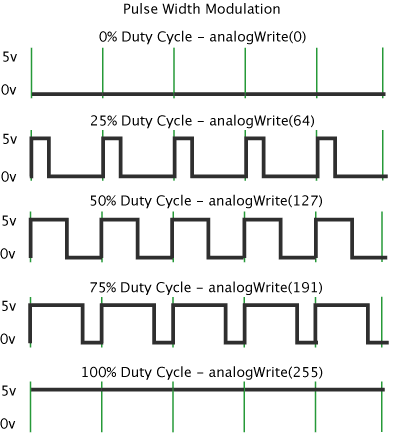
\includegraphics[scale=0.6]{images/pwm}

    \caption{How 0\%, 25\%, 50\%, 75\% and 100\% PWM is measured by a
      oscilloscop. Where Each vertical green line indicates the duty
      cycle}
    \label{fig:pwm}
  \end{nonfloatingfigure}
  
  \fixme{Better figure text and figure should be non-floating. Jesper
    has a solution to this in his old Graphics report}

  Once you get this example running, grab your Arduino and shake it
  back and forth. What you are doing here is essentially mapping time
  across the space. To our eyes, the movement blurs each LED blink
  into a line. As the LED fades in and out, those little lines will
  grow and shrink in length. Now you are seeing the pulse width.
\end{quotation}



\section{Timer Interrupts}

\fixme{fix text to support new heading: timer interrupts}

The ATmega168/ATmega328 processors has three different hardware
timers. One of them (timer 0) is used by Arduino software to provide a
\texttt{millis()} function that gives us the amount of milliseconds
since the timer started and a \texttt{delay} function that actively
holds the processor occupied for a given time period. Timer 0 and 2
uses 8 bit registers and timer 1 uses a 16 bit register. This
effectively means that timer 0 and 2 can't count to more than 255
whereas timer 1 can count to 65535. The registers is incremented at
the speed of the processor, in this case 16MHz, divided by a prescale
factor which can be either of 1 (no scaleing), 8, 64, 256, 1024 for
timer 0 and 1 and either of 1, 8, 32, 64, 128, 256, 1024 for timer
2. The reason why timer 0 and 1 has 2 less prescale factors is that
they can be wired up with an external clock source and setup to
trigger on a falling or rising edge. With a prescale of 256 the
counter is incremented at a rate of $\frac{16000000\mathrm{Hz}}{256} =
62500\mathrm{Hz}$, which makes the counter overflow at a rate of
$\frac{16000000\mathrm{Hz}}{255*256} = \frac{62500\mathrm{Hz}}{255} =
245.1\mathrm{Hz}$ (pr second). This applies to all three timers where the only
2 variables are the prescale and the size of the counter register.

The three timers modes of operation is \texttt{Normal},
\texttt{CTC}(Clear Timer on Compare match), \texttt{Fast PWM},
\texttt{Phase Correct PWM} where \texttt{Normal} and \texttt{CTC} are
the ones of interrest:

\begin{description}
\item[\texttt{Normal}] mode counts from a optionally specified counter
  value (initially default set to 0) and increments until it reaches
  the maximum value 255 where it overruns, restarts from 0, the
  interrupt is triggered and incrementation of the counter
  restarts.

\item[\texttt{CTC}] mode has a predefined top value and optionally
  specified counter value (initially default set to 0). When the
  counter reaches the defined top value it is cleared to 0, the
  interrupt is triggered and incrementation of the counter
  restarts. This gives better resolution of the counter and thus more
  flexibility than the \texttt{Normal} mode.
\end{description}

The modes of operation is described in detail in the processors
datasheet, section 12.7 ``Modes of Operation''.

\subsection{PWM generation}

PWM is generated from these three timers. Pin 5 and 6 are connected to
timer 0, 9 and 10 to timer 1 and pin 3 and 11 to timer 2. This means
that the frequency of the PWM signal is controlled by the speed of
these counters which again is determined by the prescale. When an
\texttt{analogWrite(pinnumber, value)} is executed, the value is
compared against a value in a 8-bit counter (one associated to each
timer). When the counter is less than the specified value it outputs
\texttt{HIGH} on \textit{pinnumber} and \texttt{LOW} otherwise. This
generates a square wave with a duty cycle of 50\% since it is
\texttt{HIGH} on counts $0 \ldots 127$ and \texttt{LOW} on counts $128
\ldots 255$. Since Arduino uses timer 0 for the various time related
functions, the prescale on this timer can't be changed unless this
feature are not to be used. Also because of this the duty cycle of pin
5 and 6 is not exactly the same as the other 4 pins.

\fixme{Interference problems with the PWM output pins.}  

\section{External Interrupts}

Essentially all the pins on the Arduino board supports external
interrupts, though only digital pins 2 and 3 is supported directly by
the Arduino code via the function \texttt{void attachInterrupt(int
  interruptpin, void (* userfunc)(void), int mode)} where
\textit{interruptpin} is either 0 or 1, \textit{userfunc} is the user
function to call when the interrupt triggers and \textit{mode} is one
of \texttt{LOW}, \texttt{CHANGE}, \texttt{RISING} or
\texttt{FALLING}. The \textit{mode} property is special for these two
external interrupt pins, as the other pins only support the
\texttt{CHANGE} mode. The full descriptions of the modes is in the
datasheet of the processor section 10.2.1 ``EICRA - External Interrupt
Control Register A''. To set up external interrupts on the other pins
the user \textit{ckiick} has added an usable header file to the Arduino
playground\footnote{\url{http://www.arduino.cc/playground/Main/PcInt}
  taken 28th of April 2009 at 16:45} also containing an
example of how it works. This header file defines a function
\texttt{void PCattachInterrupt(int interruptpin, void (*
  userfunc)(void), int mode)} where the only difference is that the
\textit{mode} property only supports \texttt{CHANGE}.



\section{Arduino BT}

The Arduino BT board is different from all the other Arduino boards since it
comes with a Bluegiga WT11 Bluetooth chip (from now refered to as WT11 chip)
instead of the USB mount. This means that the board can be programmed and
communicated with through a wireless connection. The communication protocol is
still RS232 so besides the wireless communication nothing is different about
this.

Other main differences as listed at the Arduino
homepage\footnote{\url{http://arduino.cc/en/Main/ArduinoBoardBluetooth} taken
  16th of May at 23:57}:

\begin{itemize}
\item The use of a DC-DC convertor, allowing the board to be powered with a
  minimum of 1.2 V, but with a maximum of 5.5 V. \textbf{Higher voltages or
    reversed polarity in the power supply will kill the board.}

\item A surface-mounted ATmega168 (as with the Arduino Mini). This doubles the
  amount of space available for your sketches and adds three more PWM pins and
  two more analog inputs.

\item Pin 7 is connected to the reset pin of the bluetooth module. 

\item Only use serial communication at 115200 baud; this is the speed that the
  module has been configured to use.
\end{itemize}

As stated digital pin 7 is reserved and connected to the WT11 chip's reset
pin. This means that if a program does a \texttt{digitalWrite(7, HIGH)} and
shortly after does a \texttt{digitalWrite(7, LOW)} the WT11 chip will be
reset. This will however not restore the factory settings of the WT11 chip as
all changes to settings are persistent.

In the below sections it is assumed that the user is using a Unix-like operating
system with Bluetooth associated packages installed, unless otherwise noted.

\subsection{Powering through a USB  cable}

As the board doesn't have the USB mount it is not able to draw power from the
host as most of the other Arduino boards has. This means that the board must be
powered by an external power supply (E.g. batteries). Powering the board when
next to a computer can however still be done through a modified USB cable. As a
standard USB cable consists of 4 wires

\begin{table}[h!]
  \centering
  \begin{tabular}{|c|c|c|}
    \hline
    Contact number & Signal name & Wire colour \\ \hline
    1 & VCC & Red \\ \hline
    2 & D- & White \\ \hline
    3 & D+ & Green \\ \hline
    3 & GND & Black \\ \hline
  \end{tabular}
  \caption{USB Connector Termination Data. Described in the USB 2.0
    specification\cite{usb20} Table 6-1 ``USB Connector Termination Assignment''}
  \label{tab:ArduinoBT:Connector_Termination_Data}
\end{table}

According to the USB 2.0 specification\cite{usb20} Table 7-7 ``DC Electrical
Characteristics'' the VCC wire supplies a minimum of 4.75v and a maximum of
5.25v which is no problem as the Arduino BT board can handle up to 5.5v and as
low as 1.2v. There is however always a slight possibility of faulty equipment
which could damage the board.

The wire colours for a standard USB 2.0 cable are defined in the
specification\cite{usb20} Figure 6-2 ``USB Standard Detachable Cable Assembly''
but it is not all manufactures that comply with this.

To construct the USB power cable all that needs done is to cut off the connector
opposite of the Standard-A connector, which is the one that fits in the
computer. Next strip off the a few cm of the PVC jacket and the copper/aluminium
shield on the cable so the four wires are free. Then cut away the 2 data wires
(green and white) and strip off 0.5cm of the VCC and GND wires insulations (red
and black). Now the two stripped wires can be connected to the Arduino BT board
through the power socket (X1). Remember not to reverse the polarity when
connecting the two wires, ore else the board cold be damaged.

\subsection{Binding with the device}

Before the board can be programmed or communicated with, it must be binded with
a host. To bind with a Bluetooth device, its MAC address is needed. A list of
names and MAC addresses of all Bluetooth devices in the area can be found with
the following command:

\begin{verbatim}
hcitool scan
\end{verbatim}

A factory Arduino BT board is always named \textit{ArduinoBT} and has the PIN
12345. There are at least 2 ways of handling Bluetooth PIN authentication. The
simplest ways is to put the PIN and nothing else in the file
\textit{/etc/bluetooth/pin} before binding with the device this however can be
complicated when binding with multiple devices with different PIN as the file
can only contain a single PIN at a time. The other way is to use
\texttt{bluetooth-applet} (Gnome) or \texttt{kbluetooth4} (KDE), which both
places a icon in the tray and queries the user for a PIN when required by the
Linux Bluetooth stack.

Whichever way is used, the host can now bind with the Arduino BT board with the
following command

\begin{verbatim}
rfcomm bind rfcommX xx:xx:xx:xx:xx:xx 1
\end{verbatim}

where \texttt{rfcommX} is the desired host device that is to be used ex
\texttt{rfcomm0}, \texttt{xx:xx:xx:xx:xx:xx} is the boards MAC Address and
\texttt{1} is the channel to be used. A factory Arduino BT board has only
enabled \texttt{SSP} (Serial Port Profile) and thus this is located on channel 1. It is
possible to query which Bluetooth profiles the Arduino BT board exposes by the
following command

\begin{verbatim}
sdptool browse xx:xx:xx:xx:xx:xx
\end{verbatim}

To find the channel, just locate \texttt{SPP} in the returned list and see what channel
the \texttt{rfcomm} protocol is associated with. 

\subsection{Important program setup}

When creating a program for the Arduino BT it is important to remember a few
things in the \texttt{setup()} function. This is to ensure that the WT11 chip is
always configured when the program starts. The WT11 chip remembers its settings even
if it loses power. This means that if the settings are change at some point of
the program execution then at least the basic settings will be set to a known
default when the program is restarted. It is however still possible to change
the settings of the WT11 chip so it won't accept connections from any
hosts. This is addressed in the below sections.

\begin{table}
  \centering
\begin{verbatim}
  pinMode(7, OUTPUT);
  Serial.begin(115200);
  digitalWrite(7, HIGH);
  delay(10);
  digitalWrite(7, LOW);
  delay(2000);

  Serial.println("SET BT PAGEMODE 3 2000 1");
  Serial.println("SET BT NAME ARDUINOBT");
  Serial.println("SET BT ROLE 0 f 7d00");
  Serial.println("SET CONTROL ECHO 0");
  Serial.println("SET BT AUTH * 12345");
  Serial.println("SET CONTROL ESCAPE - 00 1");
  Serial.println("SET CONTROL BAUD 115200,8n1");
\end{verbatim}
  \caption{asd}
  \label{tab:ArduinoBT:Initial_Setup_code}
\end{table}


The WT11 chip is connected to the Atmega chip by its RX and TX lines, which
means that communication is done through Arduino's serial communication
capabilities. The WT11 chip communicates at a baud rate of 115200 thus it is
important to use this speed in the \texttt{Serial.begin} function. Even though
the WT11 chip's iWRAP firmware can be changed to use another baud rate, this is
not recommended and will most likely not work. The name that should be visible
when searching to Bluetooth devices is configured by the \textit{SET BT NAME}
command, and the PIN is configured by\texttt{SET BT AUTH *} command. Other iWRAP
commands and their definitions can be seen in the ``iWRAP User Guide''.

\subsection{Communication with the Atmega chip without Bluetooth}

If for some reason the Arduino BT board refuses to accept connections after
binding has been done. 

\fixme{not done}

\subsection{iWRAP interface}

By default the WT11 chip uses the iWRAP firmware which enables the user to
access Bluetooth functionality with simple ASCII commands sent by a serial
interface. The Arduino BT board is shipped with the iWRAP firmware version 2.2.0
as default. If the Arduino BT board is used with a host that takes care of the
binding then there is properly no need for changing any of the WT11 chips
settings. But if the Arduino BT board is the one who needs to do the binding
with another Bluetooth device then it is necessary to change the settings and
therefor also shift into command mode. A thorough description of the different
iWRAP settings and commands can be seen in the iWRAP 2.2.0 User
Guide\cite{iWRAP220UG}.


\subsubsection{iWRAP modes}

iWRAP can be in two different modes: command mode and data mode. Before sending
any commands to the iWRAP interface it must be in command mode. The iWRAP
interface is always in command mode when there is no active connections. When
there is active connections then the mode can be switched by waiting at least
one second, sending the sequence \texttt{esc esc esc} and wait at least one
second, where \texttt{esc} is the defined escape character. When in command mode
the \texttt{SELECT} command will also change to data mode after changing the
specified connection to be the current active connection. This is discussed in
section 3 ``IWRAP MODES'' of the iWRAP 2.2.0 User Guide\cite{iWRAP220UG}.

\fixme {Mention the mux mode.}

\subsubsection{Firmaware update}

Bluegiga Technologies support 2 ways of updating the firmware. A proprietary SPI
protocol that uses a SPI interface or a open DFU (Device Firmware Update)
protocol\footnote{The DFU protocol description can be retrieved by contacting
  the Bluegiga support team.} which uses a DFU interface over a UART or USB connection.

The downside of the SPI interface is that 

\begin{itemize}
\item it requires a special SPI cable which basically is a parallel to SPI cable
  converter.

\item The proprietary BlueSuite software supplied by Bluegiga Technologies used
  to update the firmware is only released for Windows\footnote{It has not been
    confirmed whether or not it works on Linux through Wine}.

\item It is necessary to have direct access to the WT11 chip's SPI interface.
\end{itemize}

Downside of DFU interface is that 

\begin{itemize}
\item it requires special version of the firmware which can be obtained by
  contacting the Bluegiga support team.

\item It is however not all firmware versions that can be update through the DFU
  interface\footnote{``... For example iWRAP 2.1.0 can not be updated to iWRAP
    2.2.0, since the DFU boot loader code has changed''
    (\url{http://techforum.bluegiga.com/faq_item?id=10377296} 17th of may at
    19:36)}.

\item It is necessary to have access to the WT11 UART or USB
  interface. This can however be done by uploading a program to the host
  processor through Bluetooth and make it do the firmware upgrade.
\end{itemize}

Bluegiga Technologies recommends to buy or build\cite{oik_chematic} a OIK
(OnBoard Installation Kit), but the Arduino community has posted an
alternative schematic\cite{oik_chematic_arduino}.

\fixme{this section needs restructuring.}

\chapter{Guide to electronics}

\fixme{Maybe a little refresher on electronics (e.g. how each
  component are drawn in a diagram, if we are going to use diagrams in
  the article). }



\end{document}
